\chapter{Network Analysis}
\label{cap:NetworkAnalysis}
	In questo capitolo inizia la seconda parte di analisi, quella relativa alla rete. L’analisi delle reti sociali o \textit{Network Analysis} rappresenta un insieme di strumenti finalizzati a descrivere le principali caratteristiche di una struttura di nodi e connessioni rifacendosi alla teoria dei grafi. Un grafo è definito come un insieme di coppie ordinate: \\
	\verb|G=(V,A)|, \\
	dove con \verb|V| si indicano l'insieme di vertici e con \verb|A| l'insieme di archi. Un grafo può essere orientato (\textit{directed}) o non orientato (\textit{non-directed}). Nel primo caso, i legami che connettono i nodi hanno una direzionalità (in uscita da un nodo e in entrata in un altro nodo), mentre nel secondo la relazione non ha un orientamento definito. 
	
	Tramite questo tipo di rappresentazione, vedremo che è stato possibile rispondere ad alcune precise domande, grazie alle quali è stato possibile effettuare alcune strategie di \textit{marketing}, elaborare consigli per gli acquirenti e vedere il \textit{trend} di alcuni prodotti.   
	
	
	\section{Analisi sulla rete: videogiochi}
		Il nostro approccio alla rete ha riguardato il \textit{dataset} prodotti; in particolare abbiamo scelto di rappresentare un grafo per la categoria "videogiochi". L'approfondimento di questa categoria rispetto alle altre, viste nei capitoli scorsi, è stata determinata dall'intento di porre maggiormente l'attenzione su quei prodotti che avessero registrato più recensioni in assoluto, i videogiochi. 
		
		Abbiamo scelto una rappresentazione a grafo in cui i nodi fossero rappresentati dagli identificativi dei prodotti e gli archi dall'attributo \verb|also viewed| (Figura \ref{fig:network}).  Il fine del nostro studio è quello di rispondere a due principali domande: 
		\begin{itemize}
			\item \textit{Quali sono i prodotti più visti all'interno della categoria videogiochi?}
			Il primo quesito che ci siamo posti voleva essere una sorta di confronto con quanto è stato svolto durante la prima analisi, al termine della quale abbiamo ricavato una \textit{top-five} dei prodotti più recensiti, quindi nel nostro caso più popolari. Il nostro obiettivo è stato quello di andare a osservare se i prodotti più visti dagli utenti coincidano con quelli più recensiti; può infatti accadere che un prodotto, benché abbia un valore di visualizzazione molto alto, non venga poi effettivamente comprato.
			
			\item \textit{Quale prodotto per ogni sotto categoria dei videogiochi è più rilevante?}
			Durante questa analisi introduciamo il concetto di comunità, ovvero un sottoinsieme del grafo di partenza formato da nodi dalle caratteristiche simili. In particolare abbiamo deciso di raggruppare tutti i videogiochi secondo questo criterio, per comprendere sia il prodotto su cui gli utenti finisco più spesso mentre procedono nelle loro visualizzazioni.
		\end{itemize}
	
		\begin{figure} 
			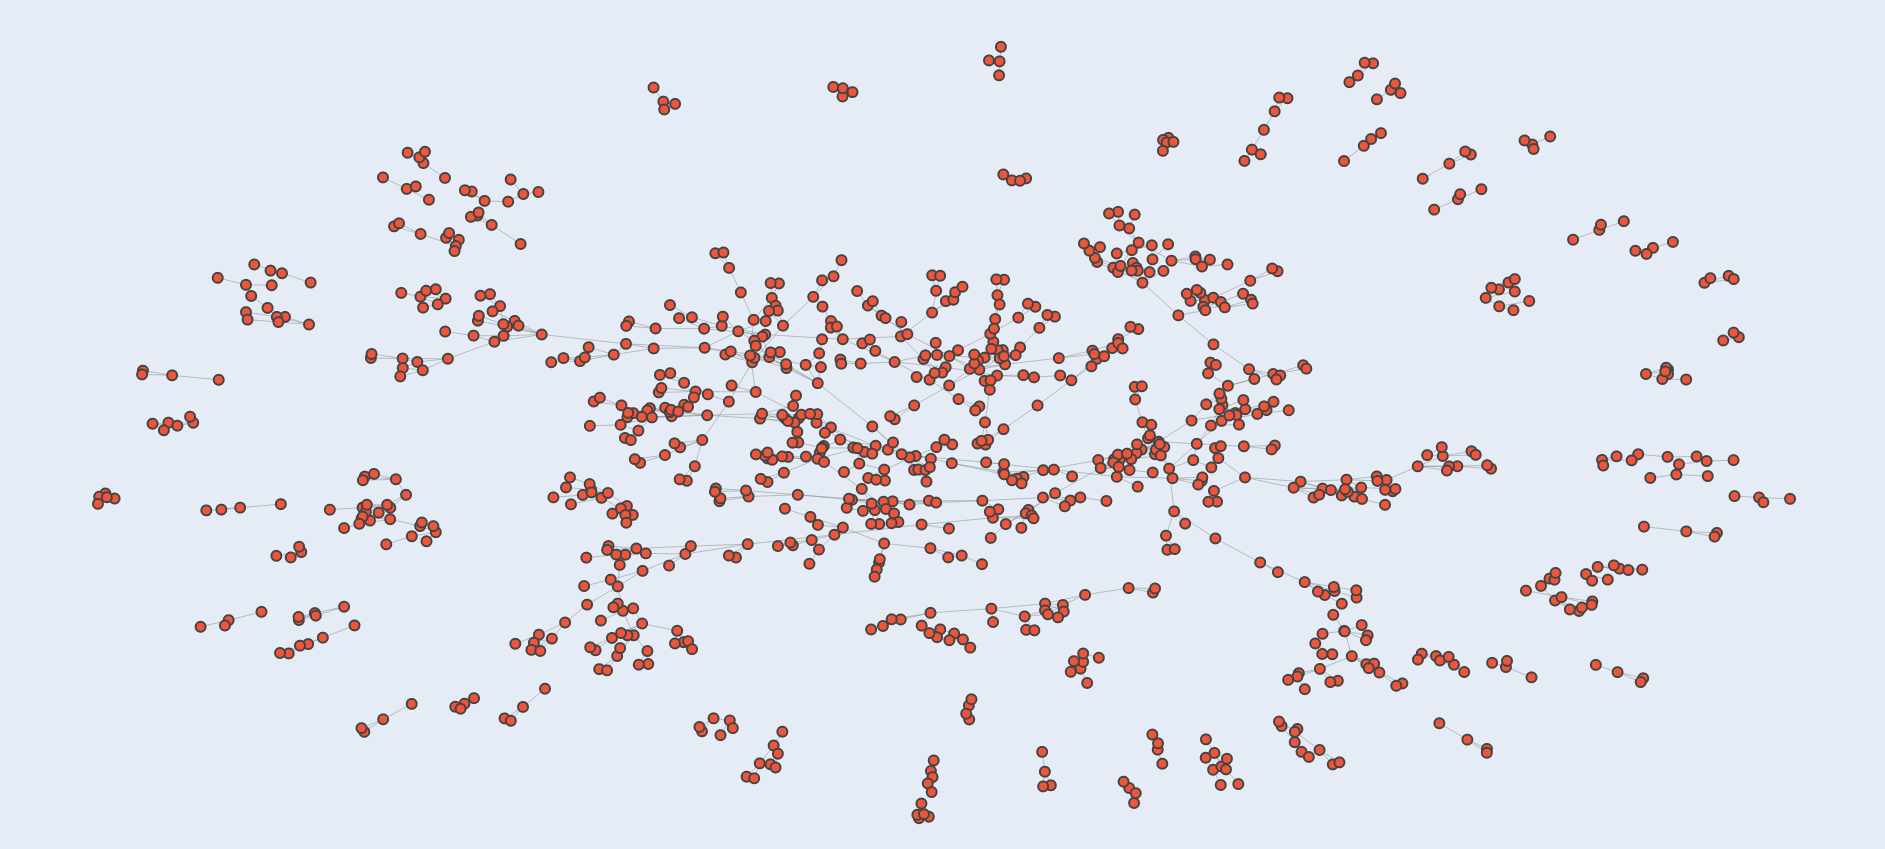
\includegraphics[width=\textwidth]{Figure/network}
			\caption{Visualizzazione della rete.}
			\label{fig:network}
		\end{figure}
		
		\subsection{Prodotti più popolari}
			Come già accennato nei paragrafi precedenti, abbiamo voluto trovare i prodotti più visto all'interno dei videogiochi e andare a confrontare i risultati con i dati rappresentati nelle Figure \ref{fig:top_pos_videogames_table}, \ref{fig:top_neg_videogames_table}. L'\textit{output} ottenuto relativo a questa è mostrato nella Tabella \ref{tab:top-five-videogames-network} ed è stato ottenuto tramite la \textit{degree centrality}, misura basata sul concetto che il nodo con più vicini è il più importante.
			
			\begin{table} [H]
				\caption{Tabella prodotti più visti: videogiochi}
				\label{tab:top-five-videogames-network}
				\centering
				\begin{tabular}{ll}
					\toprule 
					\textbf{Nome} & \textbf{Sotto categoria} \\
					\midrule
					Mario Kart 8 Deluxe & Nintendo Switch \\
					LEGO Jurassic World & PlayStation 4 \\
					Super Mario Odyssey & Nintendo Switch \\
					Nacon Revolution Pro Controller & PlayStation 4 \\
					PlayStationCamera & PlayStation 4 \\
					\bottomrule
				\end{tabular}
			\end{table}
			
			Confrontando i risultati possiamo affermare che i prodotti più recensiti nella maggior parte dei casi coincidono con quelli più recensiti, eliminando l'eccezione di "\textit{Lego Jurassic World}", che compare per la prima volta tra i più rilevanti. Un'altra considerazione può essere fatta circa la posizione dei prodotti. Alcuni di essi, infatti, slittano di qualche posizione, in alto per il caso di "\textit{Mario Kart 8 Deluxe}", verso il basso per "\textit{Super Mario Odyssey}". Una nota importante è che in questa nuova classifica troviamo i più prodotti con più recensioni positive assieme a quelli con più recensioni negative; "\textit{Nacon Revolution Pro Controller}", infatti, compariva nella Figura \ref{fig:top_neg_videogames_table}. 
		
		\subsection{Prodotti più rilevanti durante la fase di ricerca da parte di utenti}
		\label{cap:rilevantProducts}
			In questa sezione ci occuperemo di rispondere alla seconda domanda proposta. Per procedere con la nostra analisi, è stato prima di tutto necessario individuare l'insieme di tutte le sotto categorie appartenenti ai videogiochi, utilizzando il metodo \verb|Louvian|, che sarà approfondito nella sezione seguente.
		
			\begin{description}
				\item [Metodo Louvain:] è un metodo per estrarre comunità da grandi reti. L'ispirazione per questo metodo di rilevamento della comunità è l'ottimizzazione della modularità man mano che l'algoritmo progredisce. La modularità è un valore di scala compreso tra -0,5 (clustering non modulare) e 1 (clustering completamente modulare) che misura la densità relativa dei bordi all'interno delle comunità rispetto ai bordi esterni alle comunità. L'ottimizzazione di questo valore si traduce teoricamente nel migliore raggruppamento possibile dei nodi di una determinata rete, tuttavia passare attraverso tutte le possibili iterazioni dei nodi in gruppi non è pratico, quindi vengono utilizzati algoritmi euristici. Nel metodo \textit{Louvain} di rilevamento della comunità, le prime piccole comunità vengono trovate ottimizzando localmente la modularità su tutti i nodi, quindi ogni piccola comunità viene raggruppata in un nodo e il primo passaggio viene ripetuto. Il metodo è simile al metodo precedente di Clauset, Newman e Moore [3] che collega le comunità la cui fusione produce il maggiore aumento della modularità.
			\end{description}

			In seguito a questa operazione di riduzione, lo scenario che ci si presentava era composto da quasi \verb|100| comunità; numero ancora troppo elevato per rispondere al nostro quesito. La nostra scelta è stata quindi quella di raggruppare nuovamente le comunità in base al parametro \verb|console|. L'operazione ha portato all'identificazione delle seguenti \textit{community}, visibili nella Figura \ref{fig:communities}
			\begin{itemize}			
				\item Altro
				\item Nintento Switch
				\item PS4
				\item Xbox one
				\item Nintento 3DS
				\item PS3
				\item PSVita
				\item Nintento Classic Mini
				\item Nintento Wii
				\item Xbox 360
			\end{itemize}
		
			\begin{figure} [h]
				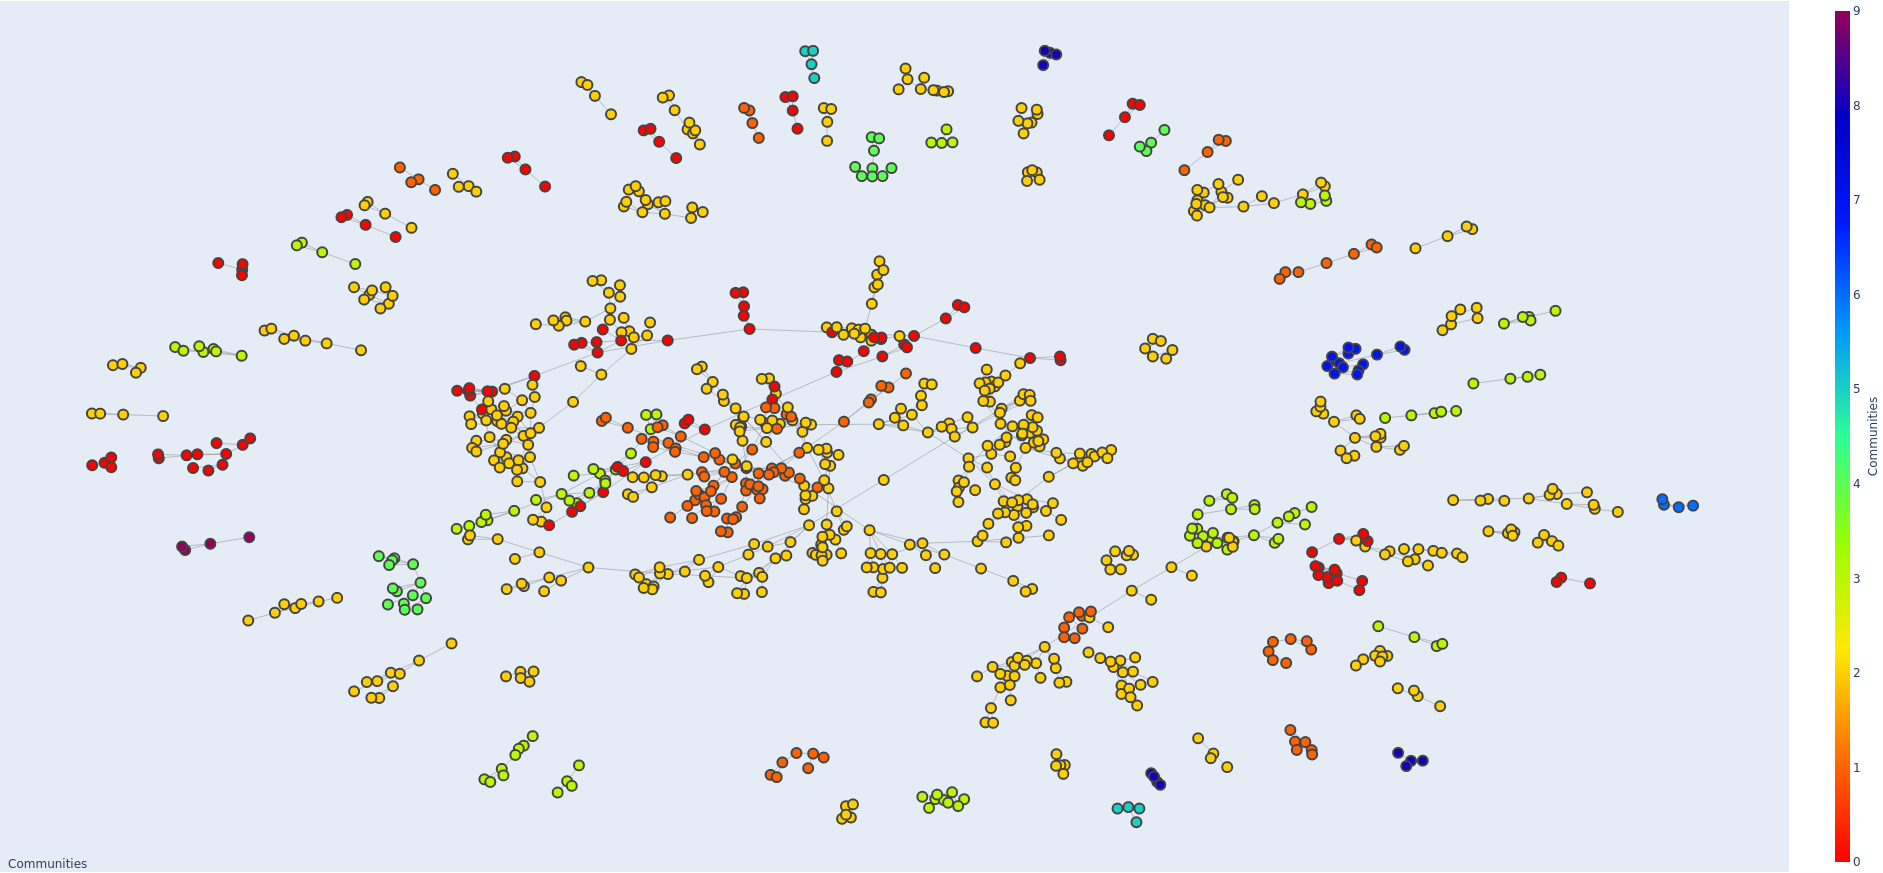
\includegraphics[width=\textwidth]{Figure/communities}
				\caption{Visualizzazione delle comunità.}
				\label{fig:communities}
			\end{figure} 
		
			All'interno di queste sotto reti abbiamo cercato il prodotto su cui gli utenti si imbattono più spesso, durante la loro procedura di ricerca. Operazione ben diversa dall'individuare quale sia il prodotto più visto in assoluto per ogni sotto insieme. Per ognuna delle nove comunità abbiamo ottenuto delle liste relative a \textit{top-five} di prodotti; queste sono visibili all'interno dell'Appendice \ref{cap:Tabelle}. L'\textit{output} ricavato è derivato dal calcolo \textit{betweness} e misura il numero di volte che un nodo agisce come ponte lungo il cammino minimo tra due nodi.
			